
%(BEGIN_QUESTION)
% Copyright 2009, Tony R. Kuphaldt, released under the Creative Commons Attribution License (v 1.0)
% This means you may do almost anything with this work of mine, so long as you give me proper credit

Suppose an electronic pressure transmitter has an input range of 0 to 100 PSI and an output range of 4 to 20 mA.  When subjected to a 5-step up-and-down ``As-Found'' calibration test, it responds as such:

% No blank lines allowed between lines of an \halign structure!
% I use comments (%) instead, so that TeX doesn't choke.

$$\vbox{\offinterlineskip
\halign{\strut
\vrule \quad\hfil # \ \hfil & 
\vrule \quad\hfil # \ \hfil \vrule \cr
\noalign{\hrule}
%
% First row
Applied pressure & Output signal \cr
%
% Another row
(PSI) & (mA) \cr
%
\noalign{\hrule}
%
% Another row
0 & 3.5 \cr
%
\noalign{\hrule}
%
% Another row
25 & 7.5 \cr
%
\noalign{\hrule}
%
% Another row
50 & 11.5 \cr
%
\noalign{\hrule}
%
% Another row
75 & 15.5 \cr
%
\noalign{\hrule}
%
% Another row
100 & 19.5 \cr
%
\noalign{\hrule}
%
% Another row
75 & 15.5 \cr
%
\noalign{\hrule}
%
% Another row
50 & 11.5 \cr
%
\noalign{\hrule}
%
% Another row
25 & 7.5 \cr
%
\noalign{\hrule}
%
% Another row
0 & 3.5 \cr
%
\noalign{\hrule}
} % End of \halign 
}$$ % End of \vbox

Sketch this instrument's ideal transfer function on the graph below, along with its {\it actual} transfer function graph based on the measured values recorded above.  Then, determine what kind of calibration error it has ({\it zero shift}, {\it span shift}, and/or {\it linearity}):

$$\includegraphics[width=15.5cm]{i00081x03.eps}$$

Finally, identify how this calibration error might be corrected.  What steps or procedures would you follow to rectify this problem?

\vskip 20pt \vbox{\hrule \hbox{\strut \vrule{} {\bf Suggestions for Socratic discussion} \vrule} \hrule}

\begin{itemize}
\item{} How might the other two calibration errors appear when graphed?
\item{} What purpose is served by doing an up-and-{\it down} test?  Why not just check the instrument's response in one direction only?
\item{} Which constant in the $y = mx + b$ linear equation represents {\it zero}, and which represents {\it span}?
\item{} Describe how a computer spreadsheet program (e.g. Microsoft Excel) might be a useful tool in graphing this instrument's response.
\end{itemize}

\underbar{file i00081}
%(END_QUESTION)





%(BEGIN_ANSWER)

This instrument has a {\it zero shift} error, but not a {\it span shift} or {\it linearity} error.

\vskip 10pt

\noindent
{\bf Ideal transfer function:}

$$\includegraphics[width=15.5cm]{i00081x01.eps}$$

\vskip 10pt

\noindent
{\bf Actual transfer function:} (zero error)

$$\includegraphics[width=15.5cm]{i00081x02.eps}$$

\vskip 10pt

\filbreak

\noindent
A span error would look something like this (wrong slope):

$$\includegraphics[width=15.5cm]{i00081x04.eps}$$

\vskip 10pt

\noindent
A linearity error would look something like this (not a straight line):

$$\includegraphics[width=15.5cm]{i00081x05.eps}$$

\vskip 10pt

A zero error is usually correctable by simply adjusting the ``zero'' screw on an analog instrument, without making any other adjustments.  Span errors, by contrast, usually require multiple adjustments of the ``zero'' and ``span'' screws while alternately applying 0\% and 100\% input range values to check for correspondence at both ends of the linear function.

%(END_ANSWER)





%(BEGIN_NOTES)

\vfil \eject

\noindent
{\bf Prep Quiz:}

Suppose an electronic pressure transmitter has an input range of 0 to 100 PSI and an output range of 4 to 20 mA.  When subjected to a series of known pressures to obtain an ``As-Found'' calibration table, it responds as such:

% No blank lines allowed between lines of an \halign structure!
% I use comments (%) instead, so that TeX doesn't choke.

$$\vbox{\offinterlineskip
\halign{\strut
\vrule \quad\hfil # \ \hfil & 
\vrule \quad\hfil # \ \hfil \vrule \cr
\noalign{\hrule}
%
% First row
Applied pressure & Output signal \cr
%
% Another row
(PSI) & (mA) \cr
%
\noalign{\hrule}
%
% Another row
0 & 4.1 \cr
%
\noalign{\hrule}
%
% Another row
25 & 8.1 \cr
%
\noalign{\hrule}
%
% Another row
50 & 12.1 \cr
%
\noalign{\hrule}
%
% Another row
75 & 16.1 \cr
%
\noalign{\hrule}
%
% Another row
100 & 20.1 \cr
%
\noalign{\hrule}
%
% Another row
75 & 16.1 \cr
%
\noalign{\hrule}
%
% Another row
50 & 12.1 \cr
%
\noalign{\hrule}
%
% Another row
25 & 8.1 \cr
%
\noalign{\hrule}
%
% Another row
0 & 4.1 \cr
%
\noalign{\hrule}
} % End of \halign 
}$$ % End of \vbox

\vskip 10pt

Identify the type of calibration error this transmitter suffers from:

\begin{itemize}
\item{} Zero shift
\vskip 5pt 
\item{} Span shift
\vskip 5pt 
\item{} Linearity
\vskip 5pt 
\item{} Hysteresis
\end{itemize}


\vfil \eject

\noindent
{\bf Prep Quiz:}

Suppose an electronic pressure transmitter has an input range of 0 to 100 PSI and an output range of 4 to 20 mA.  When subjected to a series of known pressures to obtain an ``As-Found'' calibration table, it responds as such:

% No blank lines allowed between lines of an \halign structure!
% I use comments (%) instead, so that TeX doesn't choke.

$$\vbox{\offinterlineskip
\halign{\strut
\vrule \quad\hfil # \ \hfil & 
\vrule \quad\hfil # \ \hfil \vrule \cr
\noalign{\hrule}
%
% First row
Applied pressure & Output signal \cr
%
% Another row
(PSI) & (mA) \cr
%
\noalign{\hrule}
%
% Another row
0 & 4.0 \cr
%
\noalign{\hrule}
%
% Another row
25 & 8.1 \cr
%
\noalign{\hrule}
%
% Another row
50 & 12.2 \cr
%
\noalign{\hrule}
%
% Another row
75 & 16.3 \cr
%
\noalign{\hrule}
%
% Another row
100 & 20.4 \cr
%
\noalign{\hrule}
%
% Another row
75 & 16.3 \cr
%
\noalign{\hrule}
%
% Another row
50 & 12.2 \cr
%
\noalign{\hrule}
%
% Another row
25 & 8.1 \cr
%
\noalign{\hrule}
%
% Another row
0 & 4.0 \cr
%
\noalign{\hrule}
} % End of \halign 
}$$ % End of \vbox

\vskip 10pt

Identify the type of calibration error this transmitter suffers from:

\begin{itemize}
\item{} Zero shift
\vskip 5pt 
\item{} Span shift
\vskip 5pt 
\item{} Linearity
\vskip 5pt 
\item{} Hysteresis
\end{itemize}



\vfil \eject

\noindent
{\bf Prep Quiz:}

Suppose an electronic pressure transmitter has an input range of 0 to 100 PSI and an output range of 4 to 20 mA.  When subjected to a series of known pressures to obtain an ``As-Found'' calibration table, it responds as such:

% No blank lines allowed between lines of an \halign structure!
% I use comments (%) instead, so that TeX doesn't choke.

$$\vbox{\offinterlineskip
\halign{\strut
\vrule \quad\hfil # \ \hfil & 
\vrule \quad\hfil # \ \hfil \vrule \cr
\noalign{\hrule}
%
% First row
Applied pressure & Output signal \cr
%
% Another row
(PSI) & (mA) \cr
%
\noalign{\hrule}
%
% Another row
0 & 4.0 \cr
%
\noalign{\hrule}
%
% Another row
25 & 8.1 \cr
%
\noalign{\hrule}
%
% Another row
50 & 12.2 \cr
%
\noalign{\hrule}
%
% Another row
75 & 16.1 \cr
%
\noalign{\hrule}
%
% Another row
100 & 20.0 \cr
%
\noalign{\hrule}
%
% Another row
75 & 16.1 \cr
%
\noalign{\hrule}
%
% Another row
50 & 12.2 \cr
%
\noalign{\hrule}
%
% Another row
25 & 8.1 \cr
%
\noalign{\hrule}
%
% Another row
0 & 4.0 \cr
%
\noalign{\hrule}
} % End of \halign 
}$$ % End of \vbox

\vskip 10pt

Identify the type of calibration error this transmitter suffers from:

\begin{itemize}
\item{} Zero shift
\vskip 5pt 
\item{} Span shift
\vskip 5pt 
\item{} Linearity
\vskip 5pt 
\item{} Hysteresis
\end{itemize}




\vfil \eject

\noindent
{\bf Prep Quiz:}

Suppose an electronic pressure transmitter has an input range of 0 to 100 PSI and an output range of 4 to 20 mA.  When subjected to a series of known pressures to obtain an ``As-Found'' calibration table, it responds as such:

% No blank lines allowed between lines of an \halign structure!
% I use comments (%) instead, so that TeX doesn't choke.

$$\vbox{\offinterlineskip
\halign{\strut
\vrule \quad\hfil # \ \hfil & 
\vrule \quad\hfil # \ \hfil \vrule \cr
\noalign{\hrule}
%
% First row
Applied pressure & Output signal \cr
%
% Another row
(PSI) & (mA) \cr
%
\noalign{\hrule}
%
% Another row
0 & 4.0 \cr
%
\noalign{\hrule}
%
% Another row
25 & 8.0 \cr
%
\noalign{\hrule}
%
% Another row
50 & 12.0 \cr
%
\noalign{\hrule}
%
% Another row
75 & 16.0 \cr
%
\noalign{\hrule}
%
% Another row
100 & 20.0 \cr
%
\noalign{\hrule}
%
% Another row
75 & 16.1 \cr
%
\noalign{\hrule}
%
% Another row
50 & 12.1 \cr
%
\noalign{\hrule}
%
% Another row
25 & 8.1 \cr
%
\noalign{\hrule}
%
% Another row
0 & 4.1 \cr
%
\noalign{\hrule}
} % End of \halign 
}$$ % End of \vbox

\vskip 10pt

Identify the type of calibration error this transmitter suffers from:

\begin{itemize}
\item{} Zero shift
\vskip 5pt 
\item{} Span shift
\vskip 5pt 
\item{} Linearity
\vskip 5pt 
\item{} Hysteresis
\end{itemize}

%INDEX% Calibration: basic terms and graphing
%INDEX% Calibration errors, identifying

%(END_NOTES)


